\documentclass{beamer}
\usepackage{graphics,color}
\usepackage{textcomp}
\usepackage{xcolor}
\usepackage{pgfplots}
\usepackage{pgfplotstable}
\usepackage{booktabs}
\usepackage{array}
\usepackage{colortbl}
\usepackage{amsmath,mathpazo}
\usepackage[utf8]{inputenc}
\usepackage{multicol}

\newcommand\blfootnote[1]{%
  \begingroup
  \renewcommand\thefootnote{}\footnote{#1}%
  \addtocounter{footnote}{-1}%
  \endgroup
}



\title{Buck Converter Power Train in Skywater 130nm}
\author{Teo Ene \\
  Ross Thompson}
\institute{Oklahoma State University}
\date{April 2022}

\usetheme{osu}

\begin{document}

\frame{\titlepage}

\begin{frame}
  \frametitle{Overview}
  \begin{itemize}
  \item Topology
  \item Design Parameters
  \item Circuit
  \item Deadtime
  \item Specification
  \end{itemize}
\end{frame}

\begin{frame}
  \frametitle{Topology and Design Goals}
  \begin{itemize}
  \item High efficiency voltage conversion from $3.6V$ to $1.8V$.
  \item Supply at least $400mA$.
  \item Ripple $< 40mV$
  \item Work with reasonably wide input supply $3.0$ to $4.4V$.
  \end{itemize}        
\end{frame}

\begin{frame}
  \frametitle{Passive Components and Design Selection}
  \begin{itemize}
  \item Inductor
    \begin{itemize}
    \item Part Number: SER2915L-472KL
    \item Inductance $4.7 \mu H$
    \item ESR $1.5 m\Omega$
    \end{itemize}
  \item Capacitor
    \begin{itemize}
    \item Part Number: LLL152D70J105ME01
    \item Capacitance $1\mu H$
    \item ESR $@ 1MHz$ $10 m\Omega$
    \end{itemize}
  \item Switching frequency $1Mhz$ (Found experimentally)
  \item Duty Cyle 55.5\% (Found experimentally)
  \item Nominal Output Voltage 1.8V 
  \end{itemize}
\end{frame}

\begin{frame}
  \frametitle{Buck}
  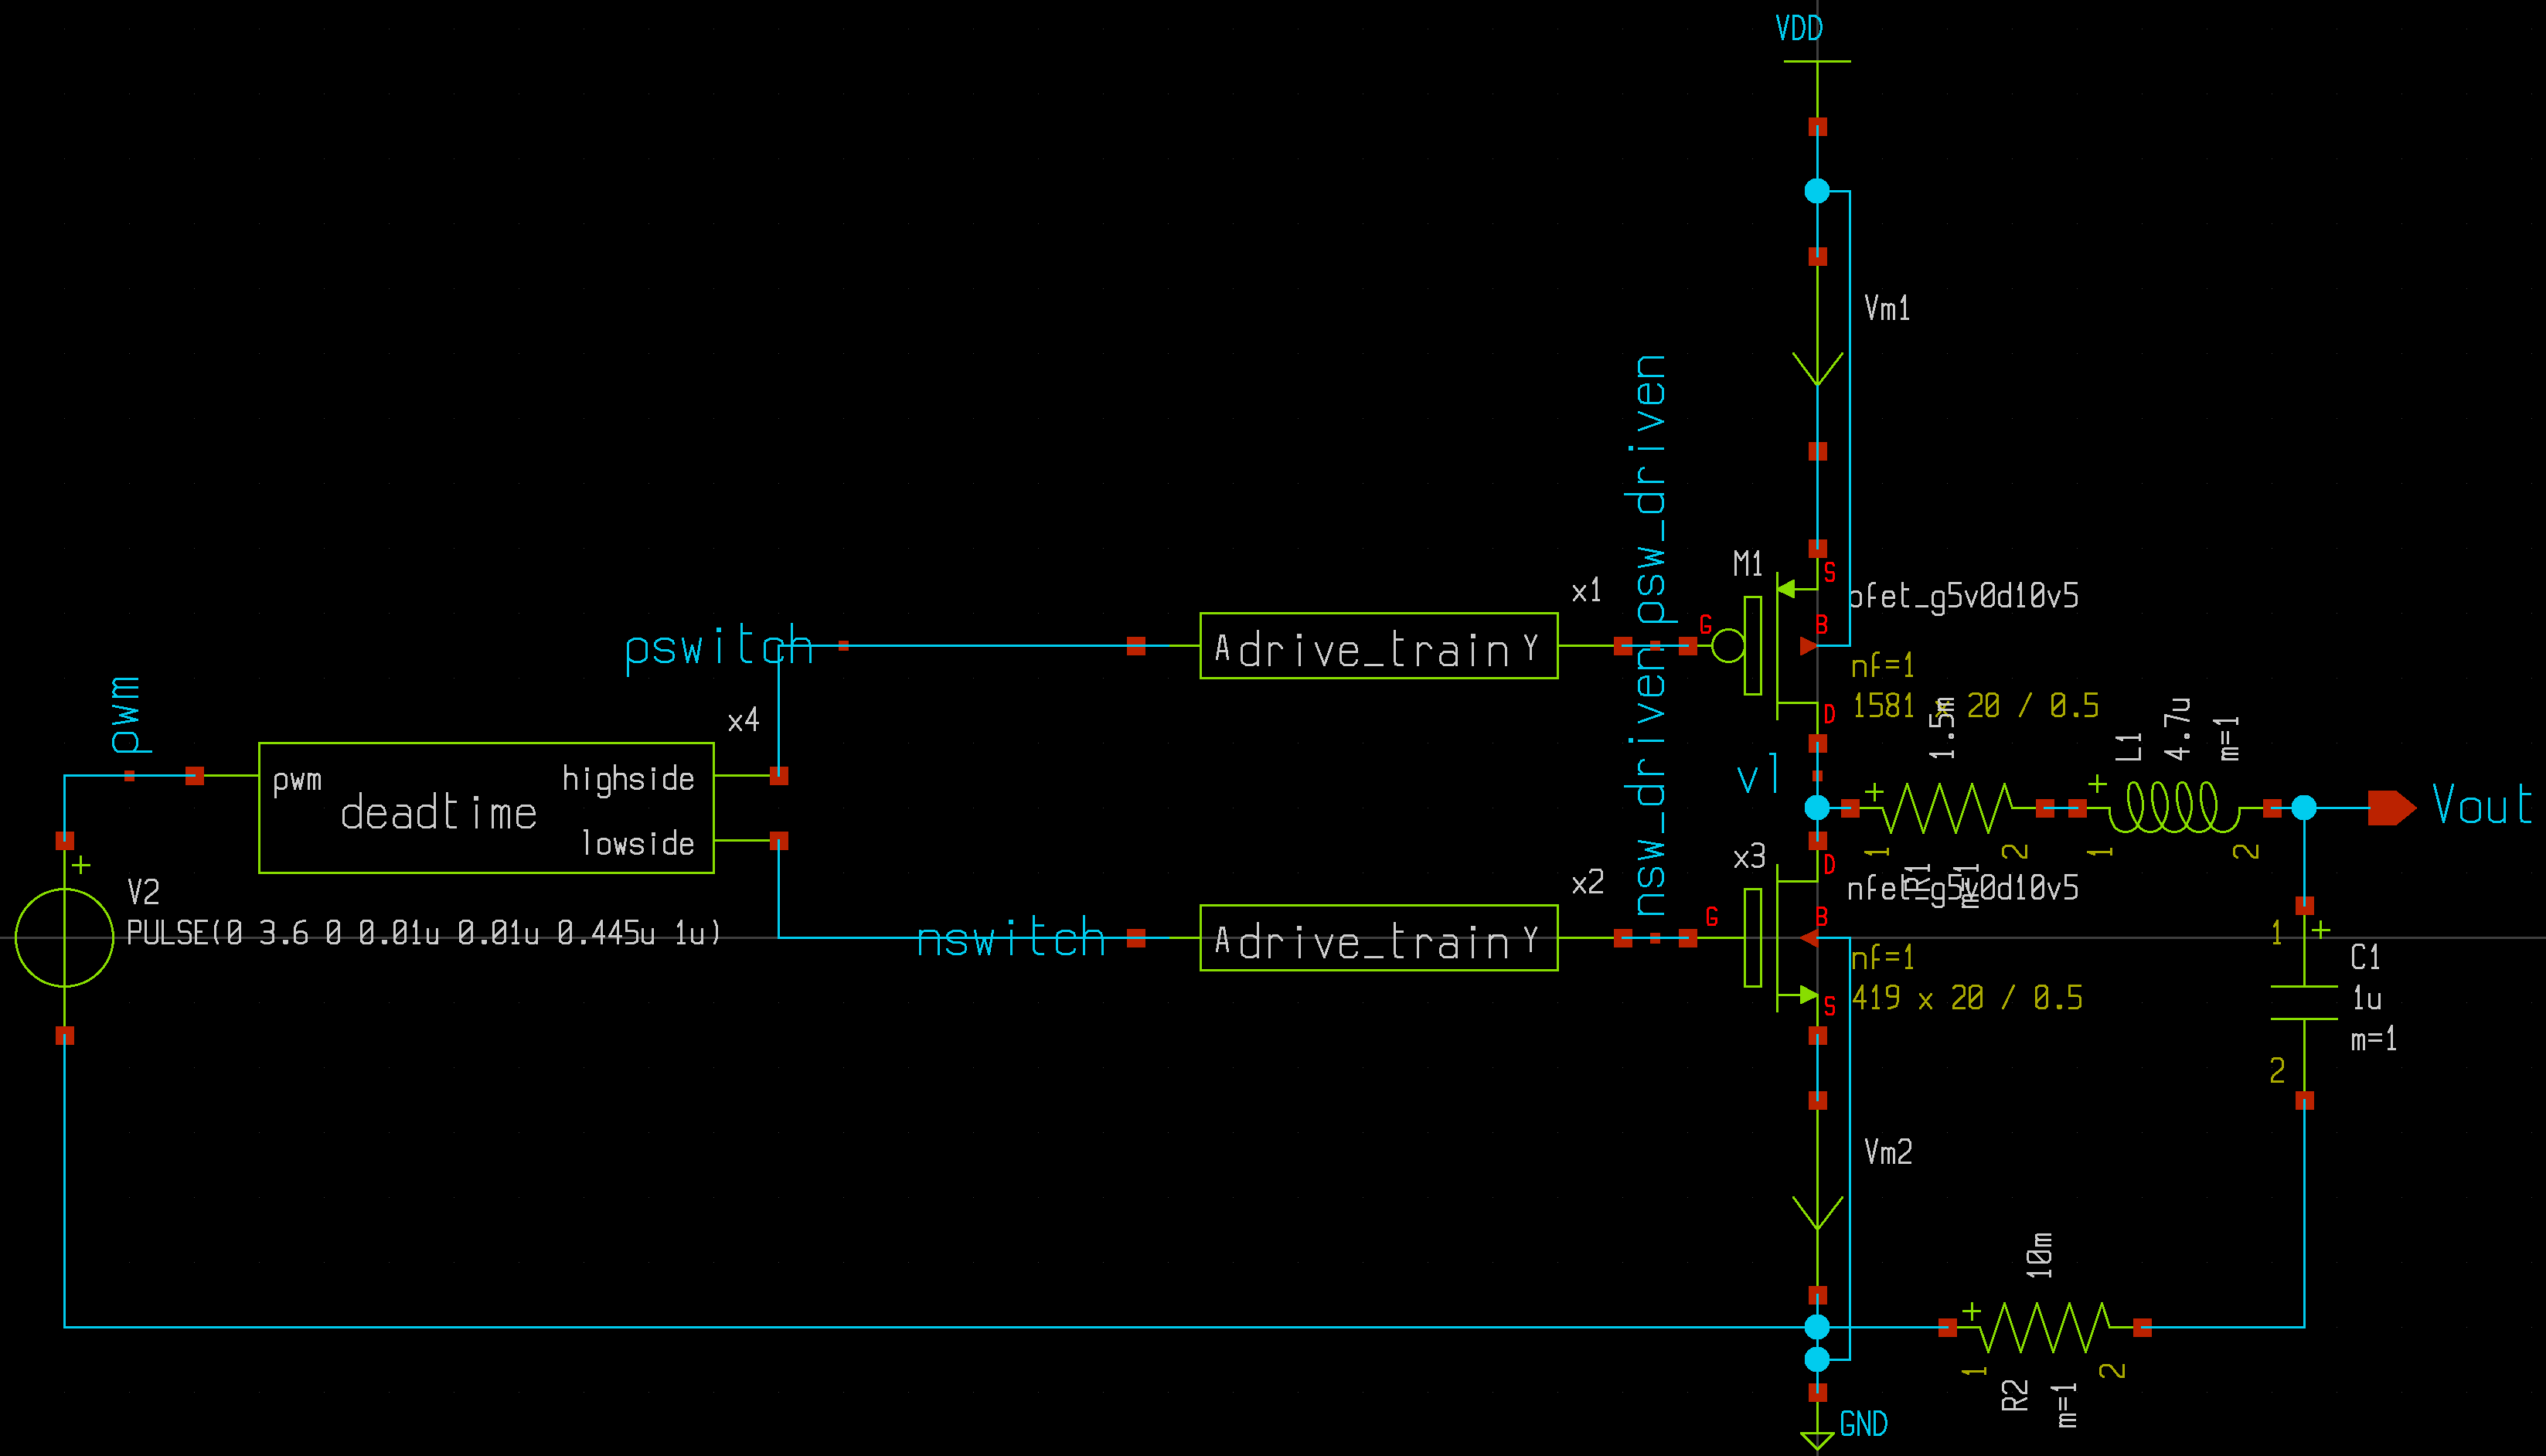
\includegraphics[scale=0.08]{buck.png}
  \begin{itemize}
  \item PMOS $W/L = 20 * 1581 / 0.5 \mu M$
  \item NMOS $W/L = 20 * 419 / 0.5 \mu M$   
  \item Total area $= 20 * (1581 + 419) * 0.5 = 20,000 \mu M^2$
  \end{itemize}
\end{frame}

\begin{frame}
  \frametitle{Power FET W/L}
  \begin{itemize}
  \item Duty Cycle of $55.5\%$ biases toward more on time for the high side.
  \item Measured Ron for an arbitrary sized PMOS and NMOS.
  \item Found the relative carrier mobility = $3.14$
  \item Including deadtime PMOS Duty Cyle $54.1\%$, NMOS $45.0\%$
  \item $54.1/45.0 = 1.202$.  $R_{onp}$ should be $1.202$ times smaller than $R_{onn}$.
  \item $W_p = 3.14 * 1.202 * W_n$
  \item PMOS $W/L = 20 * 1581 / 0.5 \mu M$
  \item NMOS $W/L = 20 * 419 / 0.5 \mu M$    
  \end{itemize}
\end{frame}

\begin{frame}
  \frametitle{Drive Train}
  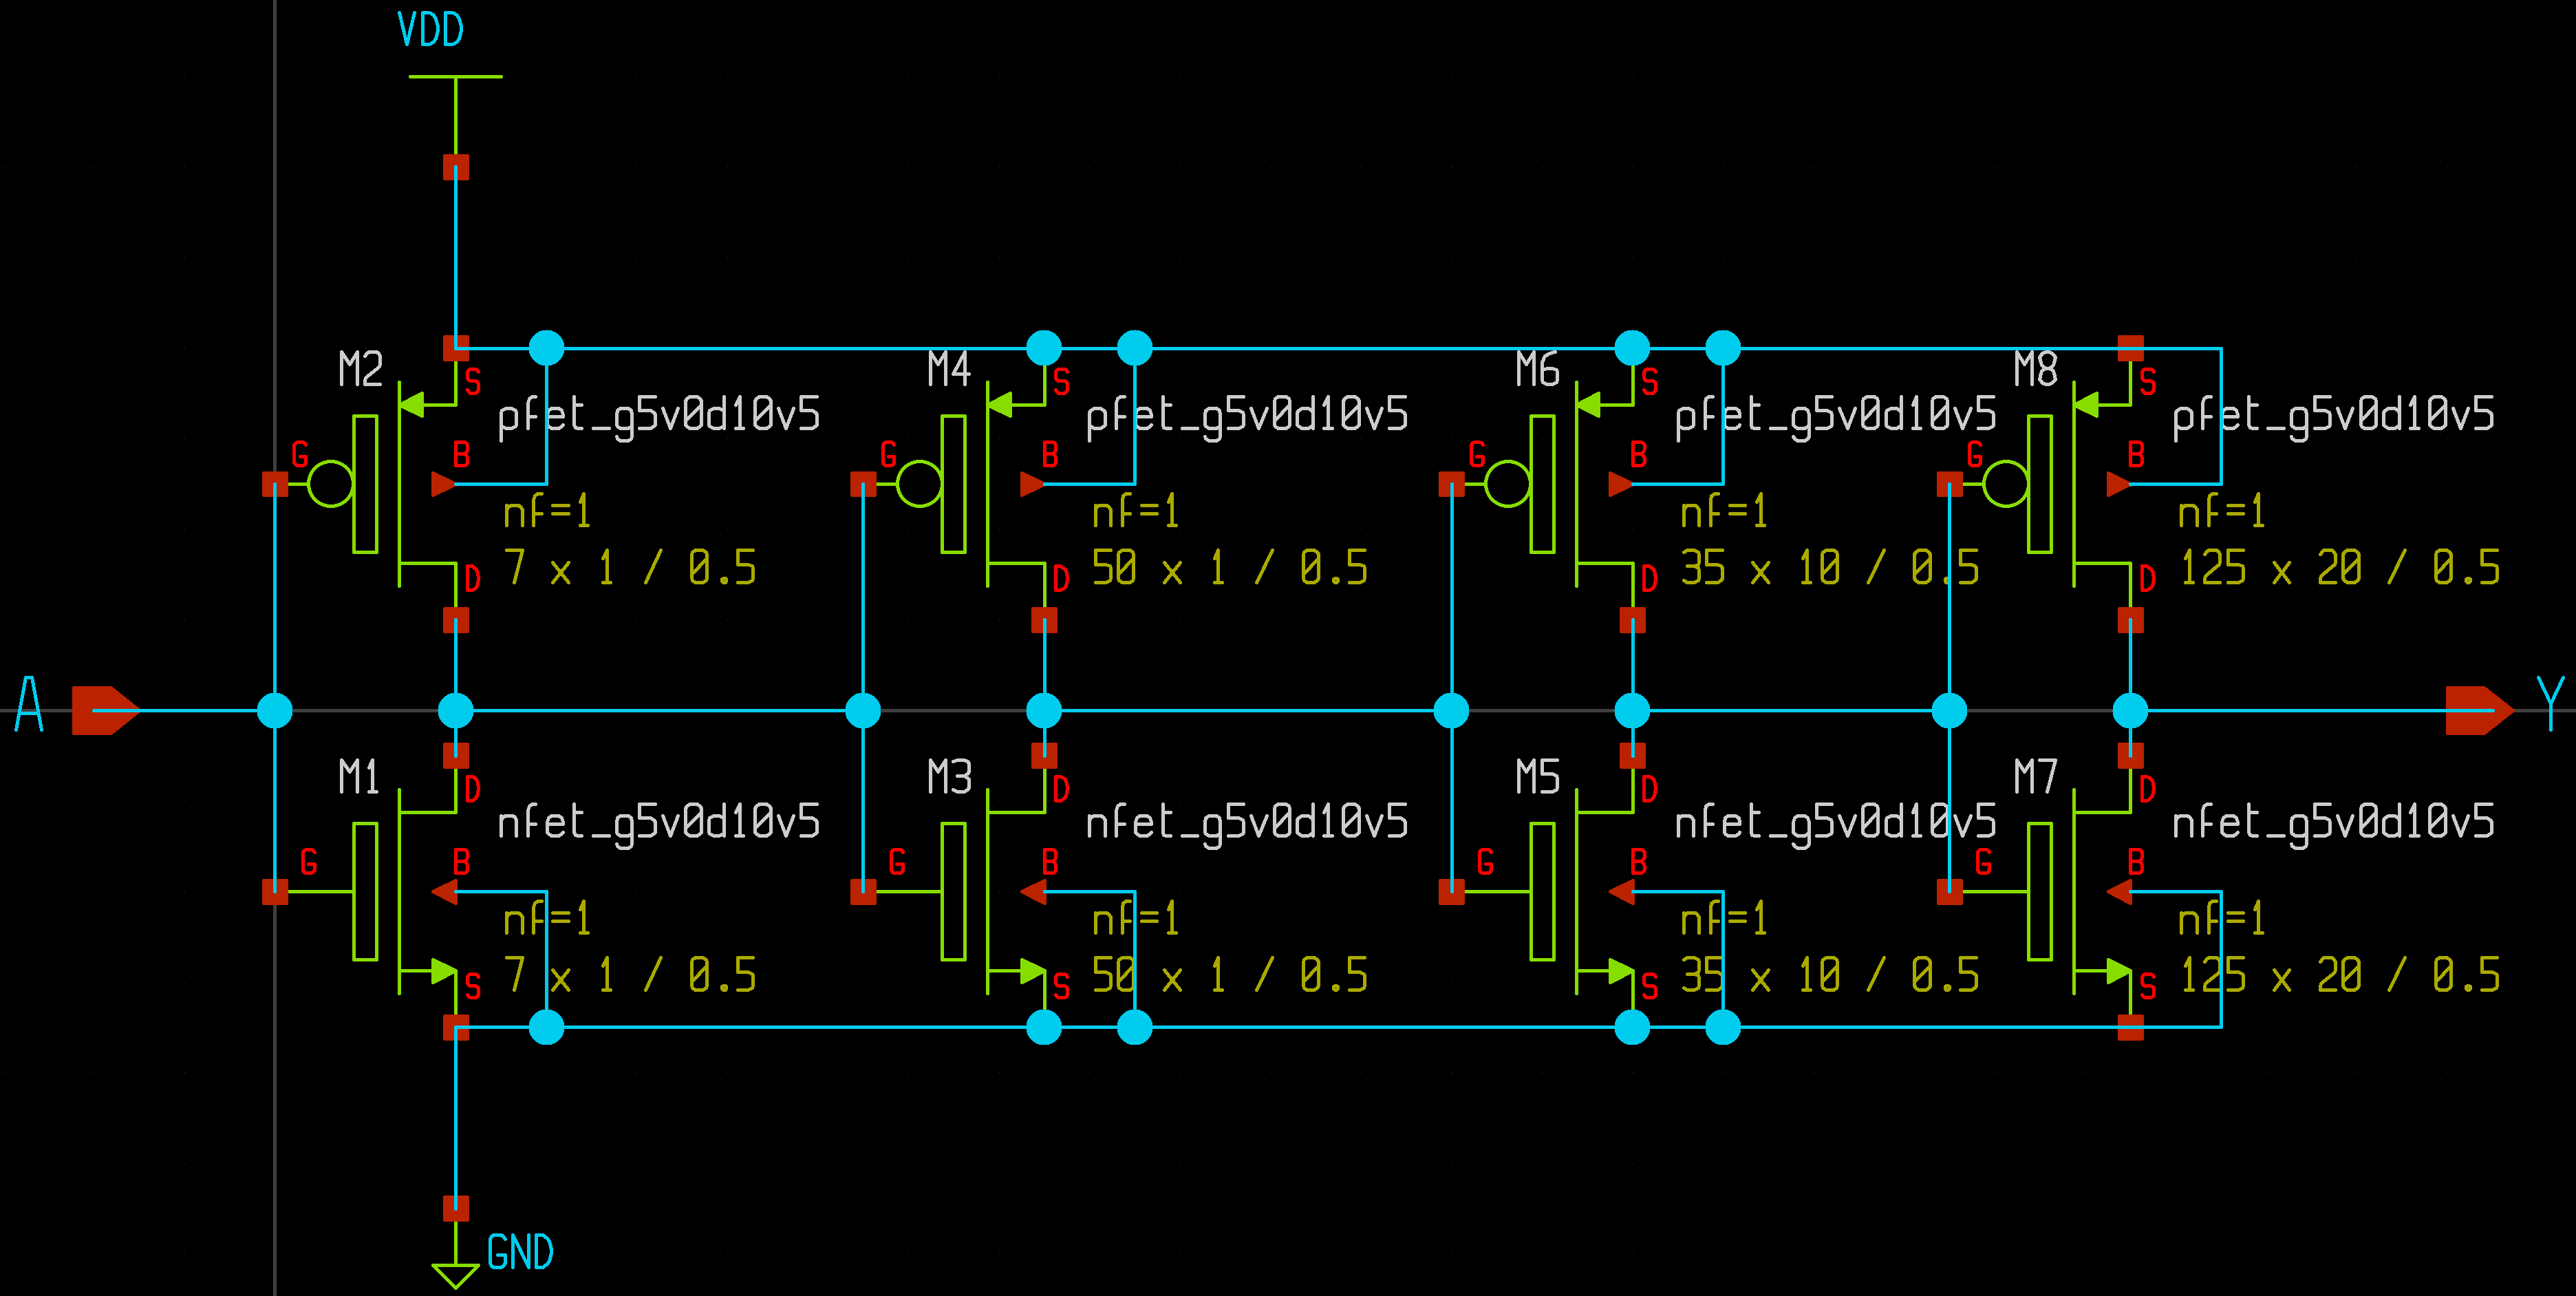
\includegraphics[scale=0.08]{drive-train.png}
  \begin{itemize}
  \item Sizes scaled in geometric series, 7, 50, 350, 2500
  \item Assumes input is 1x and output is ~20000.
  \item Total area $= (7 + 50 + 350 + 2500) * 0.5 = 1453.5 \mu M^2$
  \end{itemize}
\end{frame}

\begin{frame}
  \frametitle{Deadtime}
  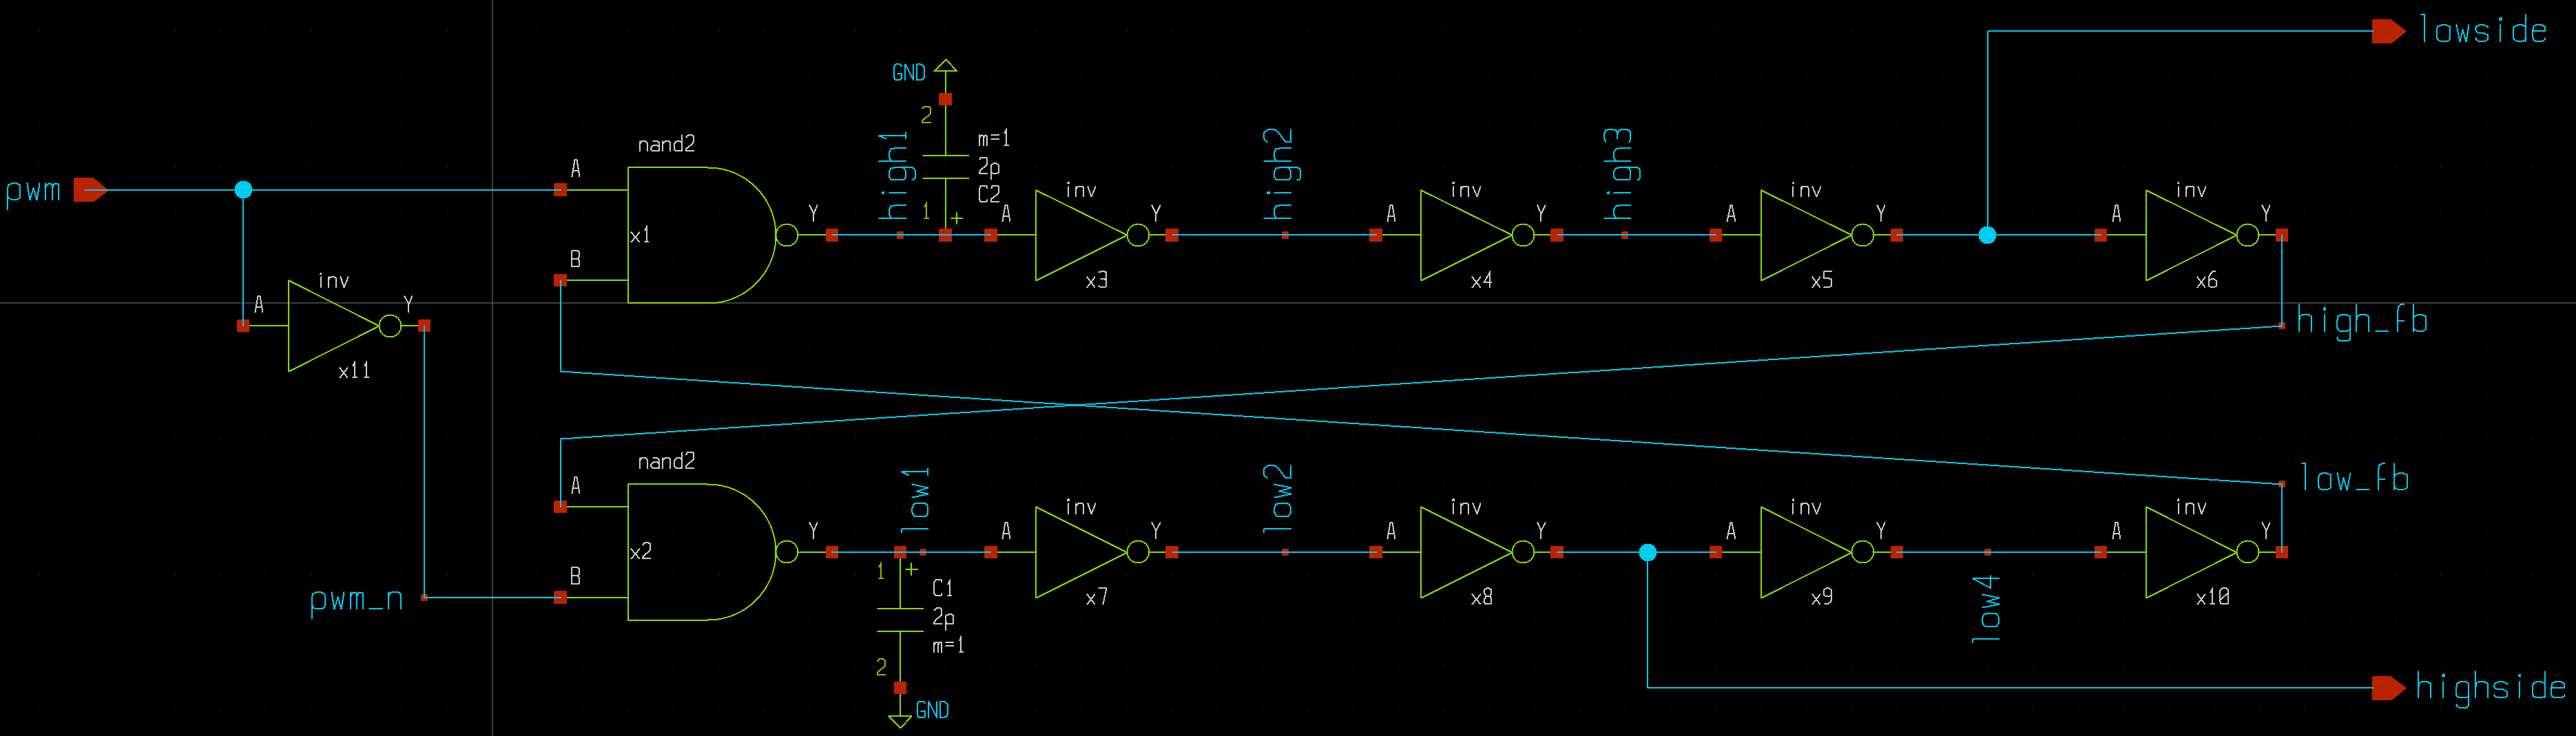
\includegraphics[scale=0.085]{deadtime.png}
  \begin{itemize}
  \item 4 chain inverter adds delay.
  \item NAND creates deadtime.
  \item 2pF cap increases propagation delay
  \item Deadtime = 15ns or 1.5\%  of period
  \end{itemize}
\end{frame}

\begin{frame}
  \frametitle{Deadtime Inverter and NAND}
  \begin{multicols}{2}
    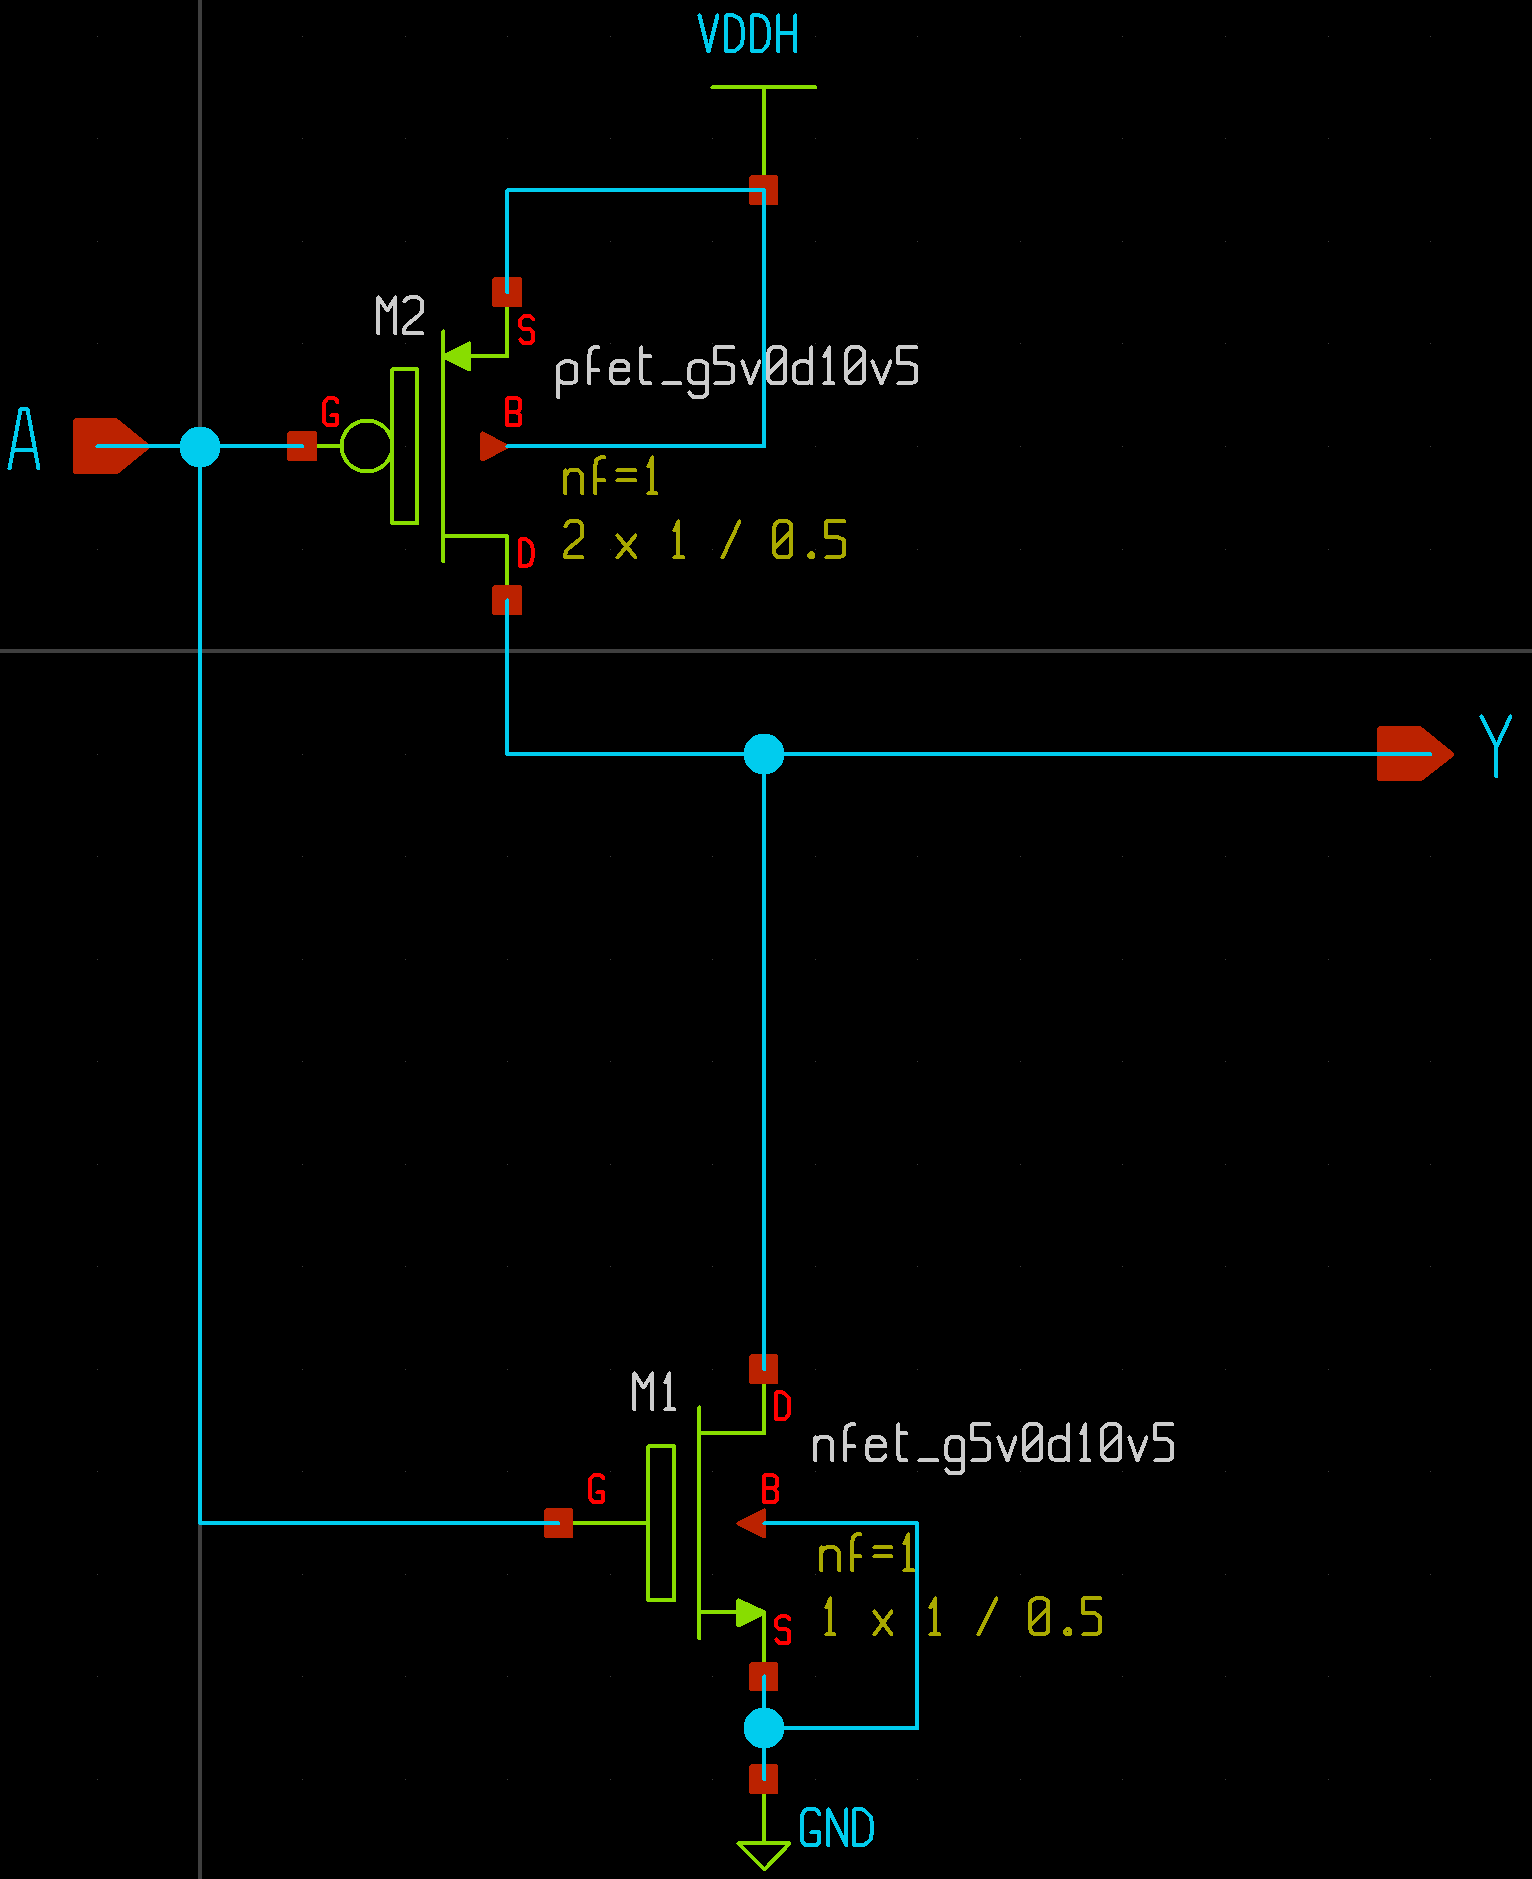
\includegraphics[scale=0.09]{inverter.png}
    \columnbreak
    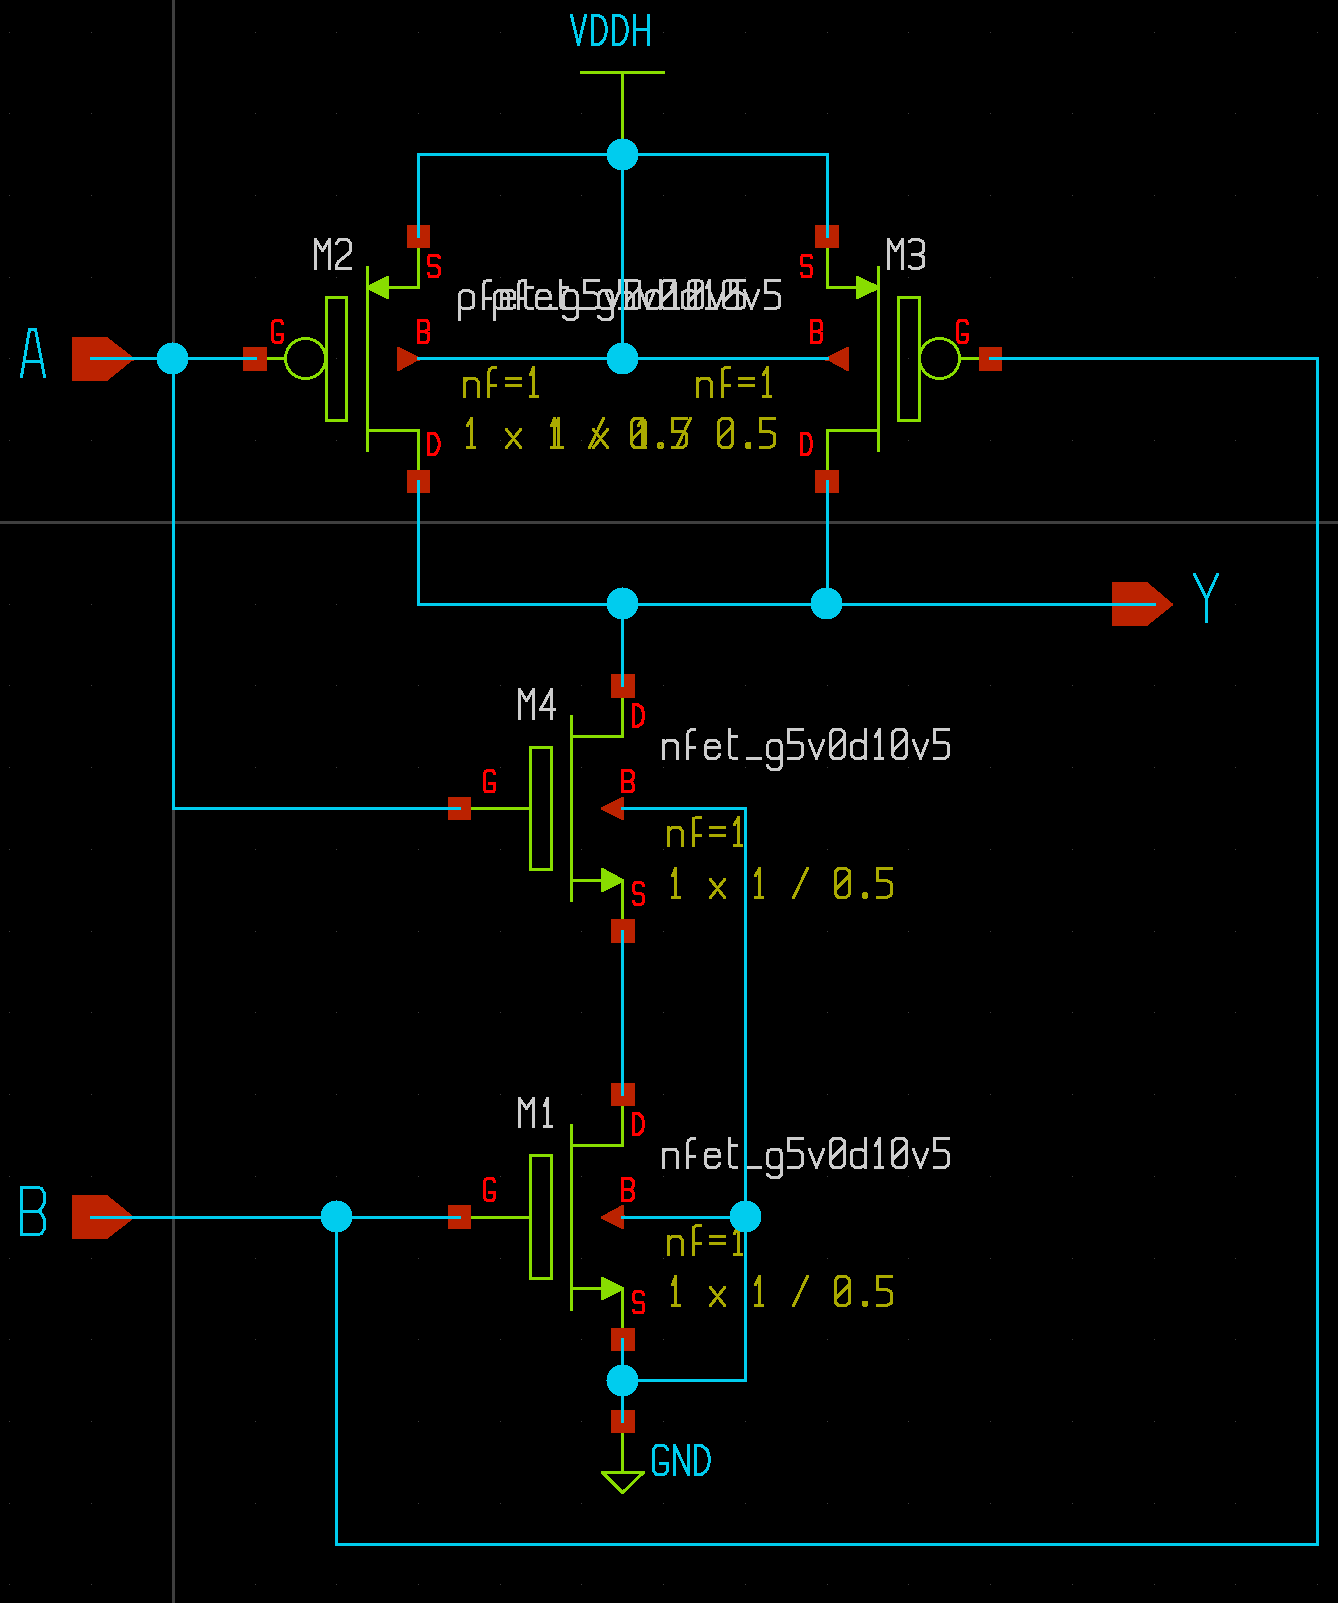
\includegraphics[scale=0.107]{nand.png}
  \end{multicols}
  \begin{itemize}
  \item Min sized 5V tolerant
  \end{itemize}
\end{frame}

\begin{frame}
  \frametitle{Test Bench}
  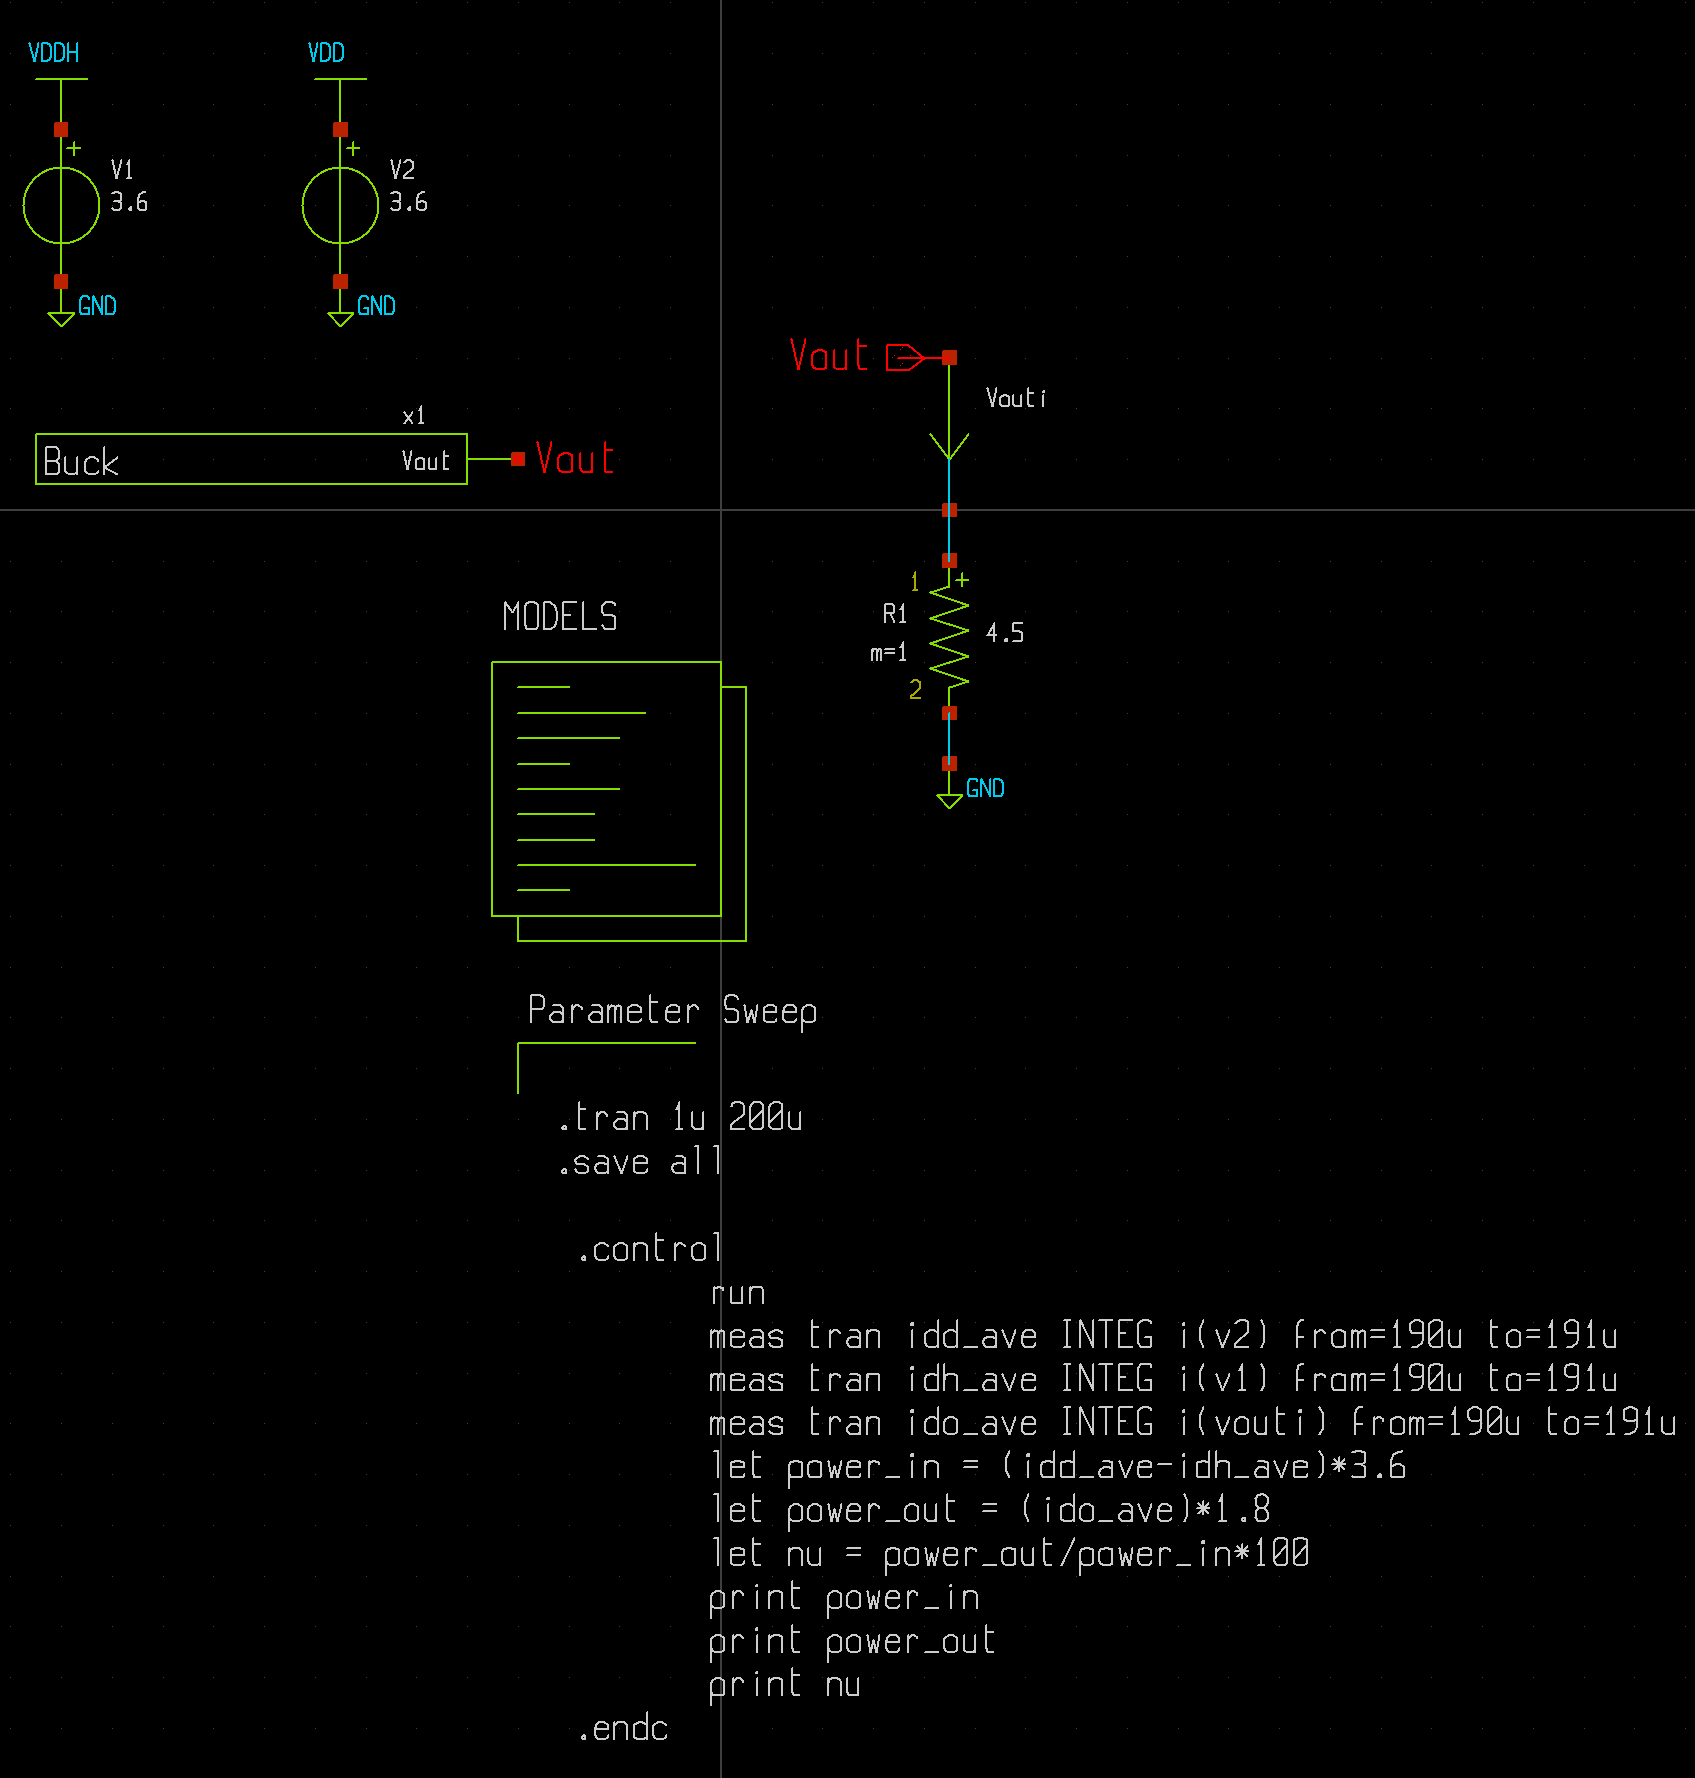
\includegraphics[scale=0.10]{testbench.png}
\end{frame}

\begin{frame}
  \frametitle{Vout at Startup }
  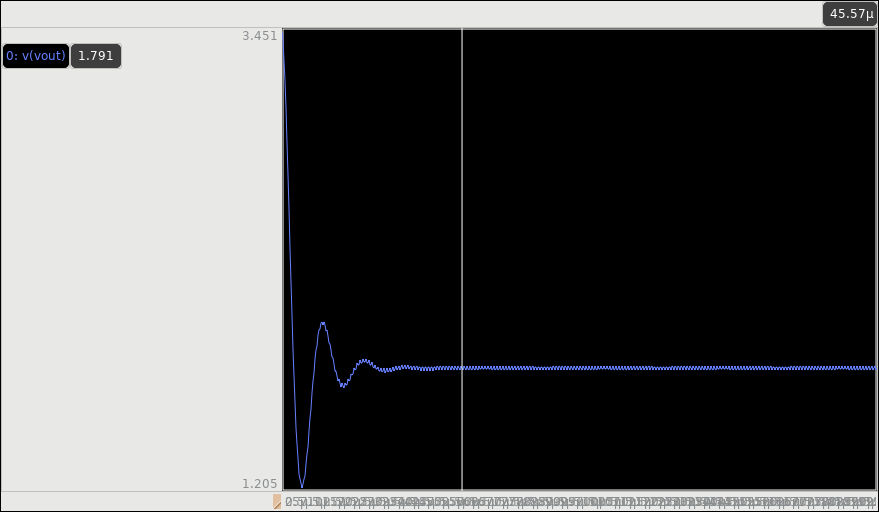
\includegraphics[scale=0.25]{startup-to-steady.png}
\end{frame}

\begin{frame}
  \frametitle{Ripple}
  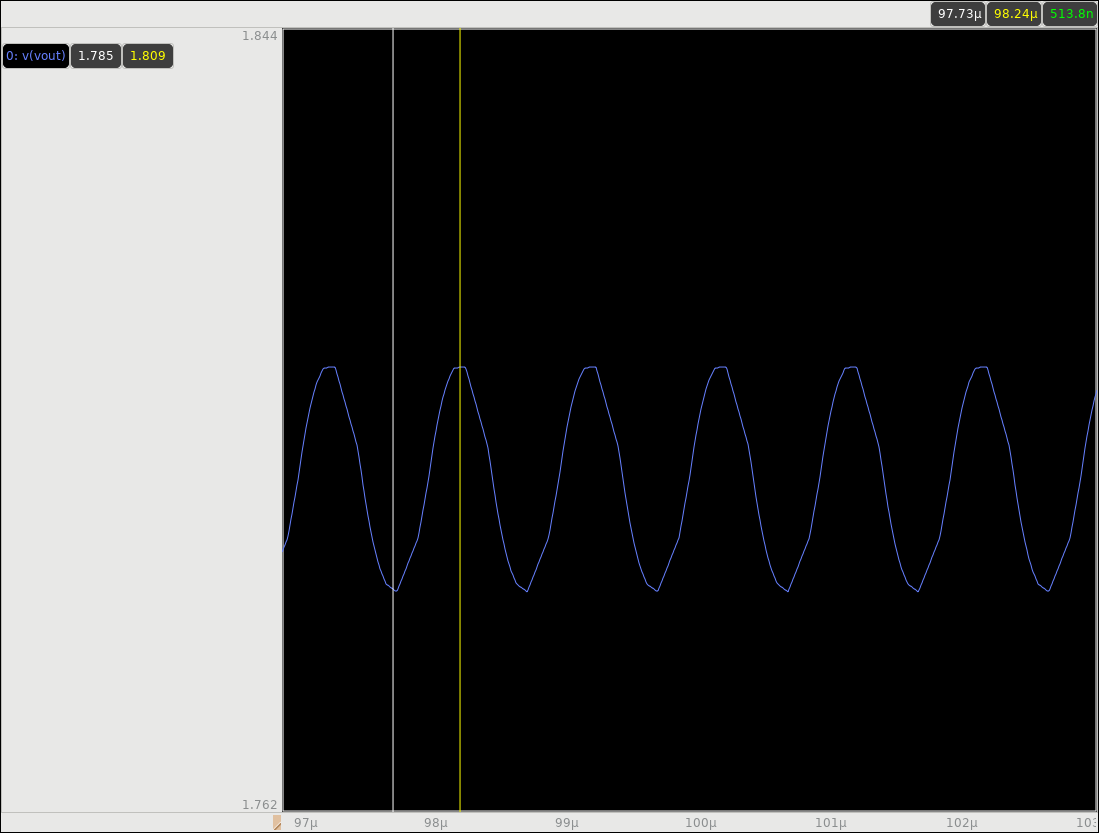
\includegraphics[scale=0.23]{ripple.png}
  \begin{itemize}
  \item $1.797 V$ DC output
  \item $24 mV$ ripple
  \end{itemize}
\end{frame}

\begin{frame}
  \frametitle{PWM input and Deadtime output at $Vin = 3.6V$}
  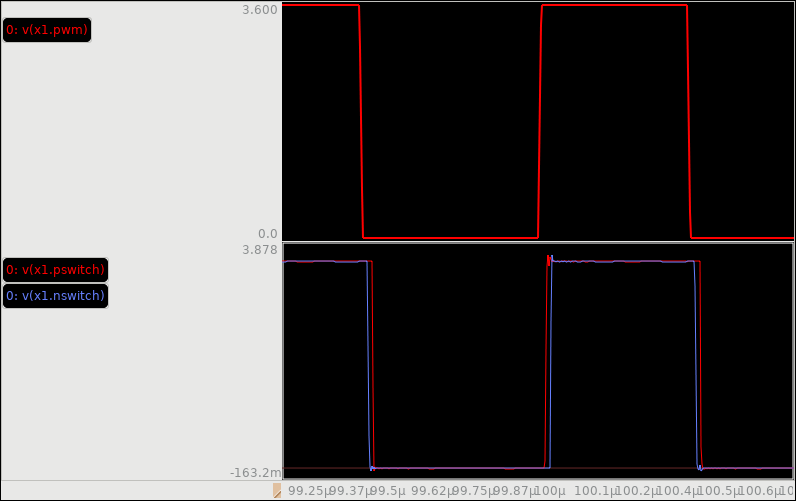
\includegraphics[scale=0.25]{pwm-deadtime.png}
  \begin{itemize}
  \item 15ns deadtime 
  \end{itemize}
\end{frame}

\begin{frame}
  \frametitle{Deadtime Measurement at $Vin = 3.6V$}
  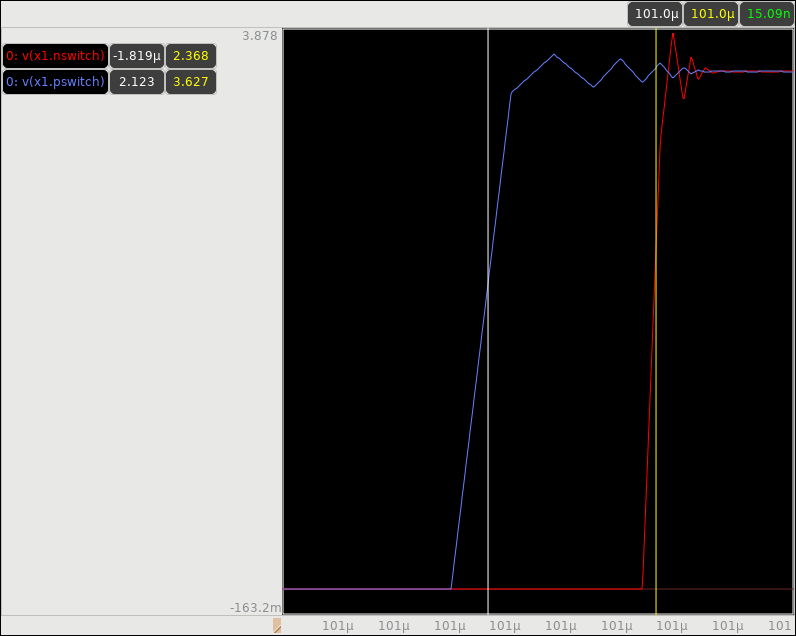
\includegraphics[scale=0.25]{pwm-deadtime-rise.png}
\end{frame}

\begin{frame}
  \frametitle{Drive Train Output $Vin = 3.6V$}
  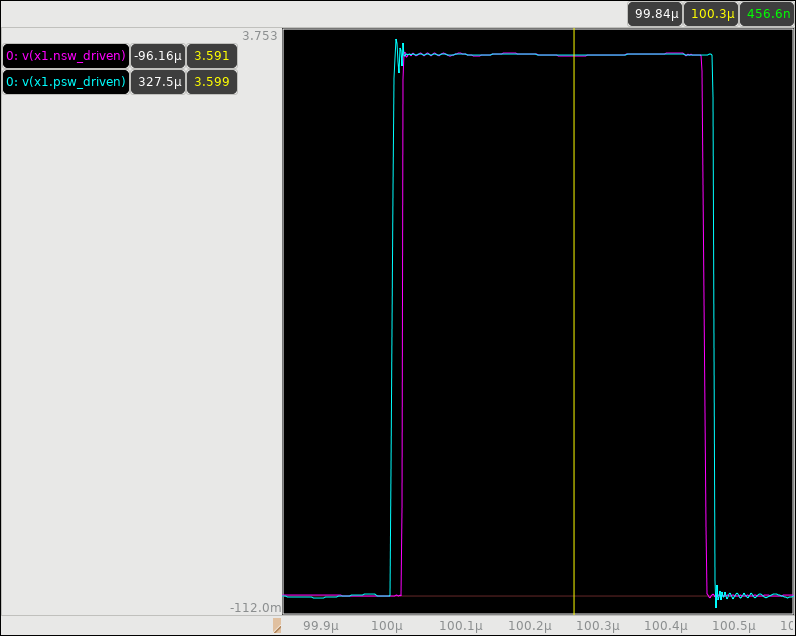
\includegraphics[scale=0.25]{drive-train-output.png}
\end{frame}

\begin{frame}
  \frametitle{Power FET Currents}
  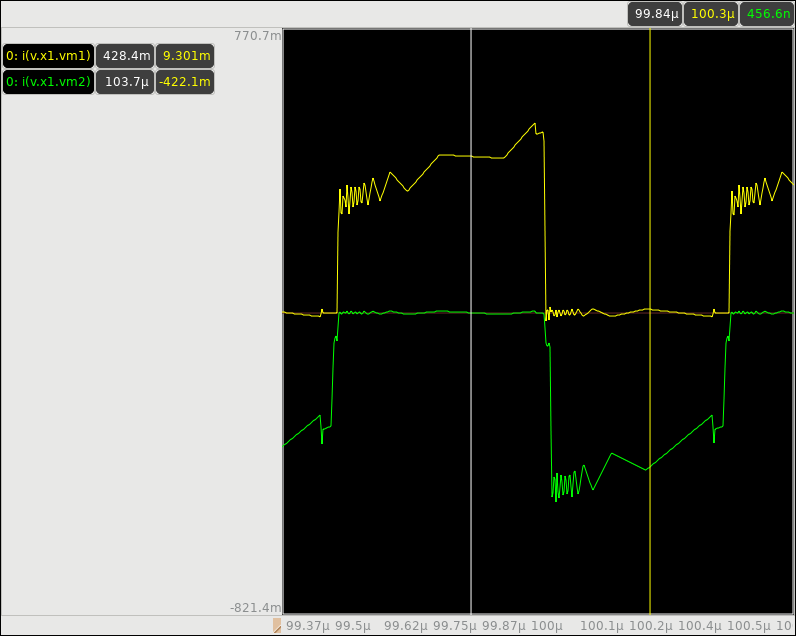
\includegraphics[scale=0.25]{hiside-lowside-current.png}
\end{frame}

\begin{frame}
  \frametitle{Compliance Matrix}
  \begin{center}
    {\scriptsize
      \begin{tabular}{| c | c | c | c | c  | c | c | c |}
        \hline      
         & \multicolumn{2}{l}{Specifications} & & \multicolumn{3}{l}{simulation results} &\\
        \hline
        Parameters & Min & Typ & Max & Min & Typ & Max & Unit \\
        \hline
        Input Voltage & 3.0 & 3.6 & 4.4 & 3.0 & 3.6 & 4.4 & V \\
        Output Voltage & & 1.8 &  & & 1.797 & & V \\
        Output Voltage Accuracy & -3 & & +3 & & 0.2 & & \% \\
        Steady state ripple p2p &  & & 40mV & & 24mV & & V \\
        Inductor & & 4.7 & & & & 4.7 & $\mu H$ \\
        Capacitor & 1 &  & 10 & & 1 & & $\mu F$ \\
        Power FET area & & & 20,000 & & 20,000 & & $\mu M^2$ \\
        Efficiency at Iout = 400mA & & & & 93.7 & 94.2 & 94.35 & \% \\
        Peak Efficiency & & & &  & 96.01 & & \% \\      
        \hline
      \end{tabular}
    }
  \end{center}

\end{frame}

\begin{frame}
  \frametitle{Efficiency vs Vin (tt) }
    \begin{tabular}{| c | c | c | c | c | c | c | c |}
        \hline
            Vin (V)  &  duty cycle &  iout (mA) &   ripple (mV) & efficiency\\\hline
            3.00 &   67.5\% &      400 &    19.7 &       93.72\%\\\hline
            3.15 &   64.5\% &      400 &    21.0 &       93.91\%\\\hline
            3.30 &   61.4\% &      400 &    22.0 &       93.99\%\\\hline
            3.45 &   58.7\% &      400 &    23.0 &       94.10\%\\\hline
            3.60 &   56.5\% &      400 &    23.8 &       94.23\%\\\hline
            3.75 &   54.4\% &      400 &    25.0 &       94.28\%\\\hline
            3.90 &   52.3\% &      400 &    25.6 &       94.36\%\\\hline
    \end{tabular}
\end{frame}

\begin{frame}
  \frametitle{Efficiency vs Vin (tt) }
  \includegraphics[scale=0.6]{vin-eff.pdf}
\end{frame}

\begin{frame}
  \frametitle{Ripple vs Vin (tt)}
  \includegraphics[scale=0.6]{vin-ripple.pdf}
\end{frame}

\begin{frame}
  \frametitle{Peak Efficiency vs Iout}
  \includegraphics[scale=0.6]{io-eff.pdf}
  $max: 96.01\%$ at $Iout = 100 mA$
\end{frame}

\begin{frame}
  \frametitle{Efficiency vs Iout}
    \begin{tabular}{| c | c | c | c | c | c | c | c |}
        \hline
            Vin (V) &    duty cycle &   iout (mA) &   ripple (mV) & efficiency\\\hline
            3.60 &   42.2\% &800 &    24.0 &      90.30\%\\\hline
            3.60 &   43.6\% &530 &    23.8 &      92.91\%\\\hline
            3.60 &   44.5\% &400 &    23.8 &      94.23\%\\\hline
            3.60 &   45.0\% &300 &    23.8 &      95.15\%\\\hline
            3.60 &   45.6\% &200 &    24.0 &      96.00\%\\\hline
            3.60 &   46.4\% &100 &    23.8 &      96.01\%\\\hline
            3.60 &   49.0\% &10  &    23.6 &      80.28\%\\\hline
            3.60 &   48.7\% &1   &    25.4 &      27.90\%\\\hline
    \end{tabular}
\end{frame}

\begin{frame}
  \frametitle{Ripple vs Iout}
  \includegraphics[scale=0.6]{io-ripple.pdf}
  $max: 25.4 mV$ at $Iout = 10 mA$
\end{frame}

\begin{frame}
    \begin{center}
      \frametitle{Sufficient Load for Continuous Conduction}
      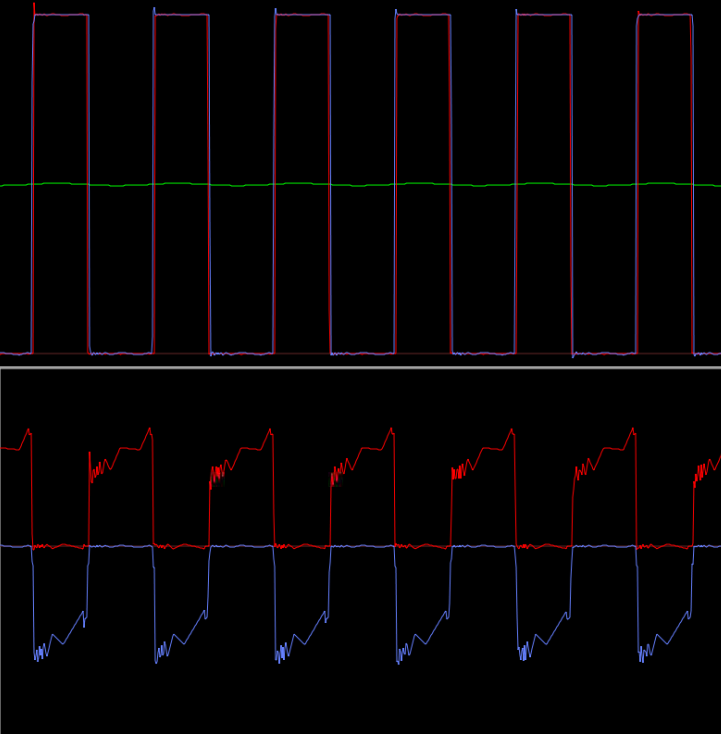
\includegraphics[scale=0.3]{buck_working.png}
    \end{center}
\end{frame}

\begin{frame}
    \begin{center}
      \frametitle{Insufficient Load for Continuous Conduction}
      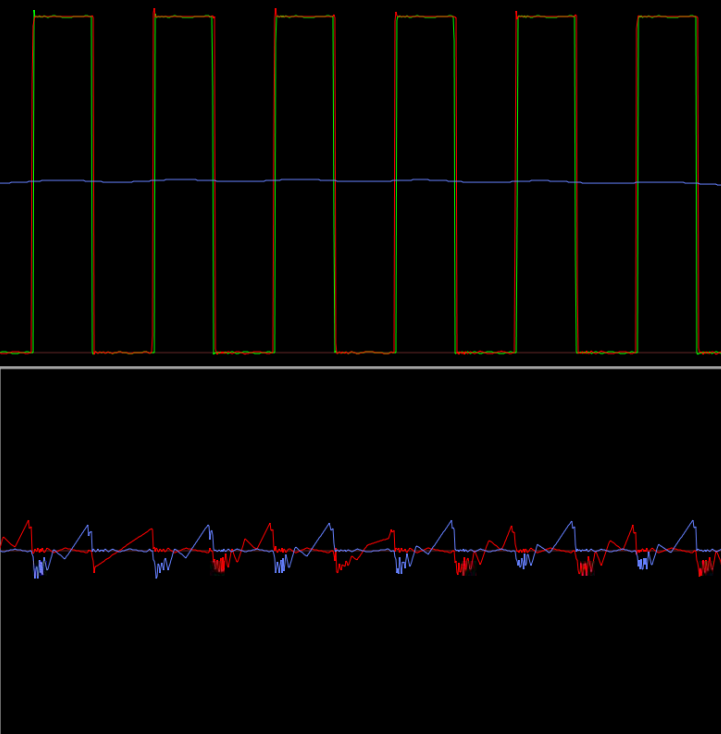
\includegraphics[scale=0.3]{buck_not_working.png}
    \end{center}
\end{frame}

\end{document}
